\documentclass[11pt,letterpaper]{article}
\usepackage[utf8]{inputenc}

%----- Configuración del estilo del documento------%
\usepackage{epsfig,graphicx}
\usepackage[left=2cm,right=2cm,top=1.8cm,bottom=2.3cm]{geometry}
\usepackage{fancyhdr}
\usepackage{lastpage}

\usepackage{xcolor}
\usepackage{soul}
\newcommand{\mathcolorbox}[2]{\colorbox{#1}{$\displaystyle #2$}}

%Color bibi
\definecolor{bibi}{RGB}{0,103,148}
% Otros colores

%------ Paquetes de dibujo --------%
\usepackage{tikz}
\usepackage{circuitikz}

%------ Paquetes para mantener las imágenes en su lugar --------%
\usepackage{float}

%------ Paquete para notacion de dirac -------%
\usepackage{braket}

%------ Paquete para reescribir los enumitems -------%
\usepackage{enumitem}

\usepackage{cite}
\usepackage{multicol}
\setlength{\columnsep}{1.5cm}
\setlength{\columnseprule}{.5pt}

\pagestyle{fancy}
\fancyhf{}
\rfoot{\textit{Página \thepage \hspace{1pt} de \pageref{LastPage}}}

%------ Paquetes matemáticos básicos --------%
\usepackage{amsmath}
\usepackage{amssymb}
\usepackage{amsthm}

\begin{document}
%------ Encabezado -------- %
\begin{center}
    \begin{minipage}{3cm}
    	\begin{center}
    		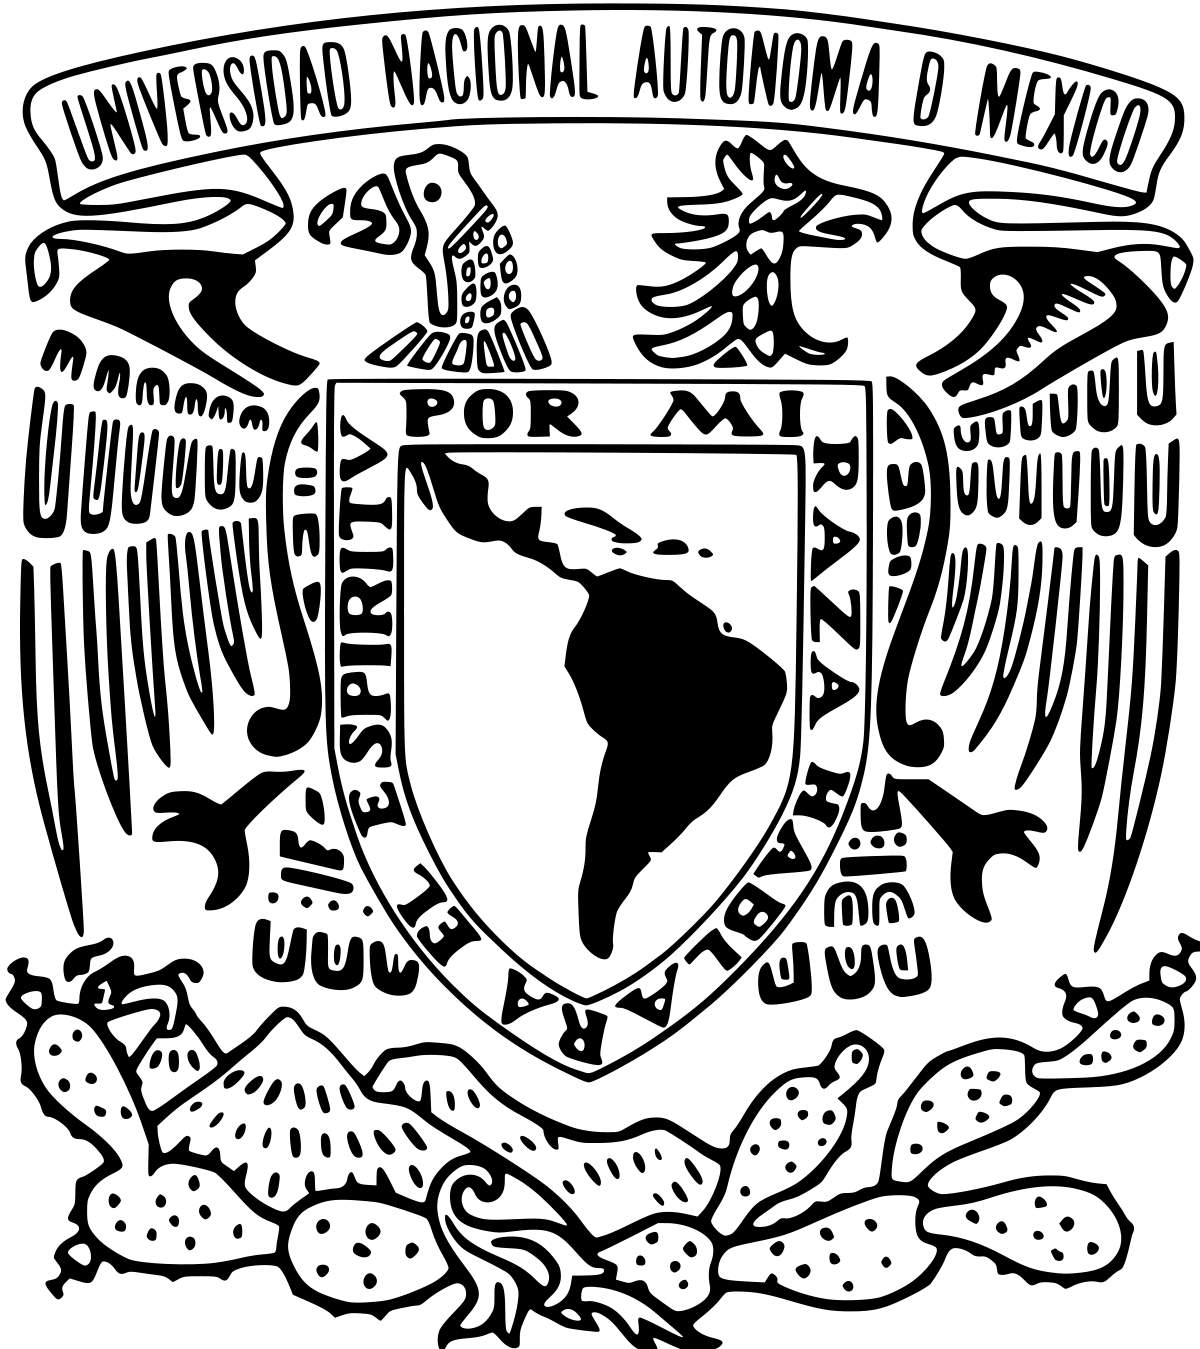
\includegraphics[height=3.3cm]{src/Img/Logo_UNAM.png}
    	\end{center}
    \end{minipage}\hfill
    \begin{minipage}{10cm}
    	\begin{center}
    	\textbf{\large Universidad Nacional Autónoma de México}\\[0.1cm]
        \textbf{Facultad de Ciencias}\\[0.1cm]
        \textbf{Análisis de Algoritmos  $|$ 7083}\\[0.1cm]
        Tarea 3 : $|$ Programacion Dinamica\\[0.1cm]
        Sosa Romo Juan Mario $|$ 320051926 \\[0.1cm]
        25/09/24
    	\end{center}
    \end{minipage}\hfill
    \begin{minipage}{3cm}
    	\begin{center}
    		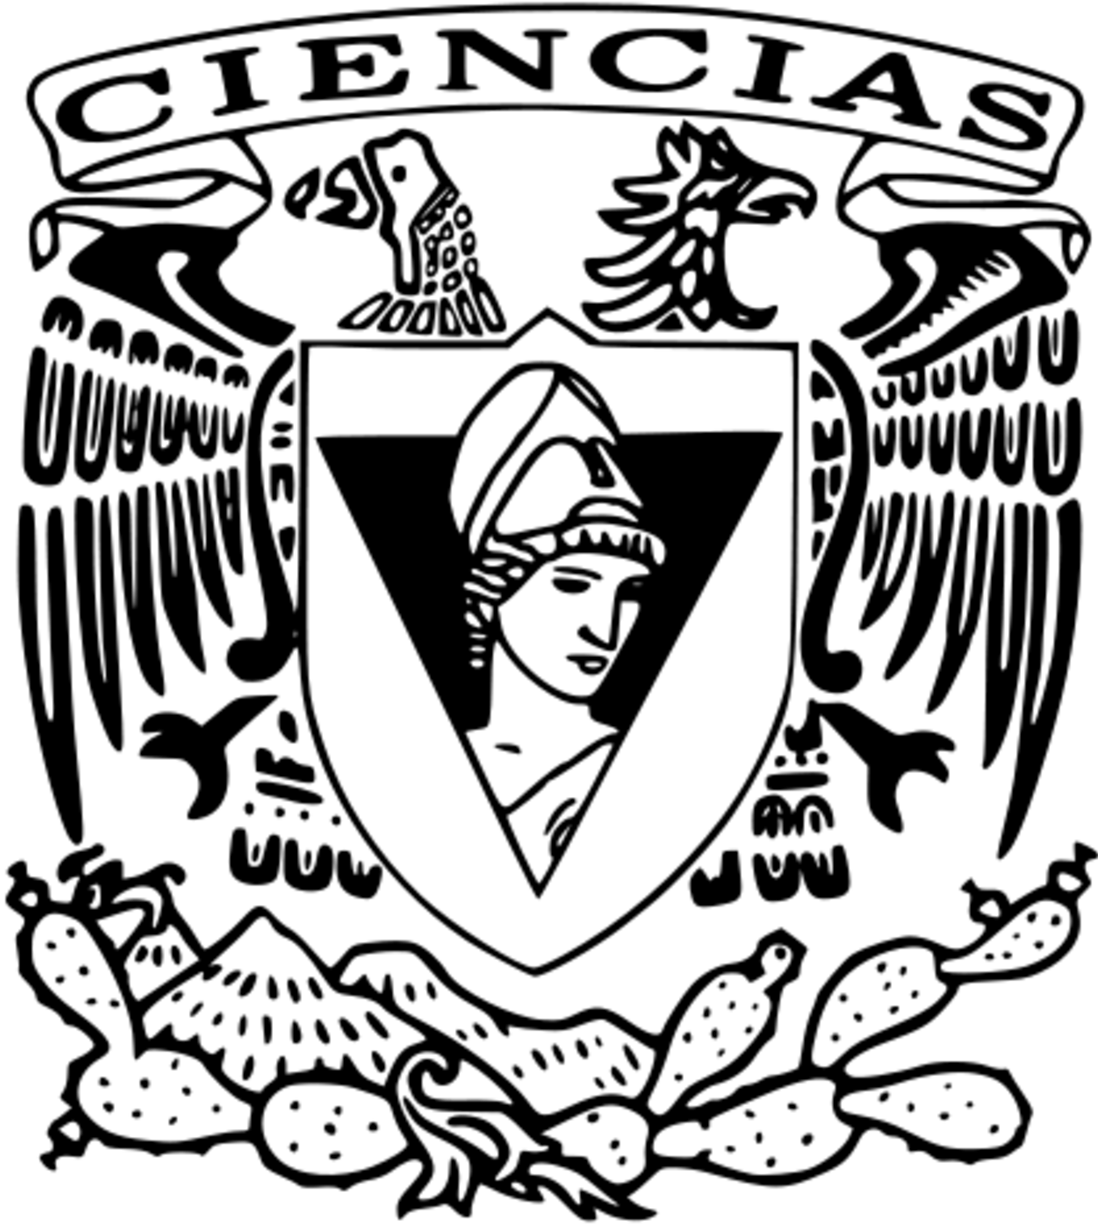
\includegraphics[height=3.3cm]{src/Img/Logo_FC.png}
    	\end{center}
    \end{minipage}
\end{center}


\rule{16.99cm}{0.1mm}

%------ Ejercicios -------- %
\begin{enumerate}
    \item \textbf{Basado en las notas del curso, por favor calcula el protocolo de
teletransportación cuántica usando el estado de Bell $\ket{\beta}_{02}$}\vspace{.2cm}

\[
    \ket{\beta_{02}} = \displaystyle\frac{\ket{01}+\ket{10}}{\sqrt{2}}  
\]

\textbf{Y el estado $\ket{psi}$ a ser teletransportado definido como:}
\[
    \ket{\psi} = \alpha \ket{0} + \beta{1}  
\]

\textbf{Puedes basarte de la fig1 para seguir visualmente el protocolo.}
 
\begin{center}
    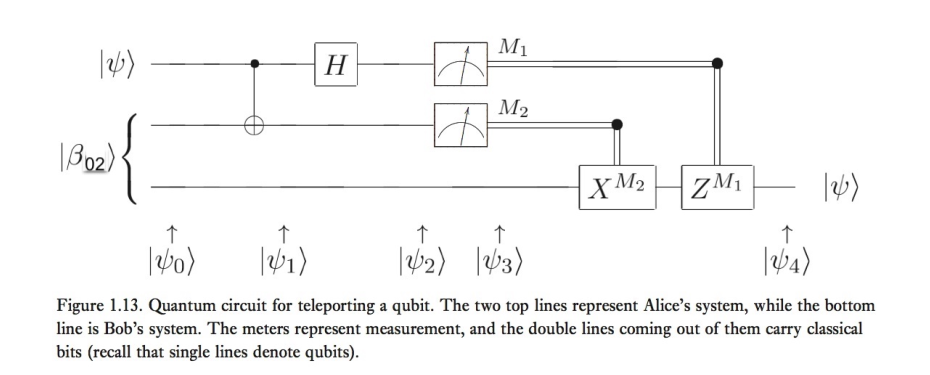
\includegraphics[height=6cm]{src/Img/1.png}
\end{center}

    \begin{enumerate}
        \item \textbf{Por favor deriva con procedimiento los siguientes estados cuánticos:
$\ket{\psi}_0, \ket{\psi}_1$, $\ket{\psi}_2\ket{\psi}_3$ y $\ket{\psi}_4$.}\vspace{.2cm}

\textcolor{bibi}{Siguiendo las notas del curso}\vspace{.2cm}

\begin{itemize}
    \item $\mathbf{\ket{\psi_0}}$ \vspace{.3cm}
        
        Calculamos el estado de los 3 qubits antes de operar:

        \begin{align*}
            \ket{\psi_0} &= \ket{\psi} \otimes \ket{\beta_{02}} \\
            &= (\alpha\ket{0} + \beta\ket{1}) \otimes
            \left(\frac{\ket{01}+\ket{10}}{\sqrt{2}}\right)\\
            &=
            \mathcolorbox{yellow}{\frac{1}{\sqrt{2}}\left(\alpha\ket{001}+\alpha\ket{010}+\beta\ket{101}+\beta\ket{110}\right)}\\
        \end{align*}        

    \item $\mathbf{\ket{\psi_1}}$\vspace{.3cm}

        Aplicamos $C_{NOT}$ a los primeros 2 qubits e $\mathbb{I}$ al tercero:

        \begin{align*}
            \ket{\psi_1} &= \hat{C}_{NOT} \otimes \hat{\mathbb{I}} \ket{\psi_0} \\
            &= (\hat{C}_{NOT} \otimes \hat{\mathbb{I}})
            \left(\frac{1}{\sqrt{2}}\left(\alpha\ket{00}\ket{1}+\alpha\ket{01}\ket{0}+\beta\ket{10}\ket{1}+\beta\ket{11}\ket{0}\right)\right)
            \\
            &= \frac{1}{\sqrt{2}}\left(\alpha\ket{00}\ket{1}+\alpha\ket{01}\ket{0}+\beta\ket{11}\ket{1}+\beta\ket{10}\ket{0}\right)
            \\
            &=\mathcolorbox{yellow}{\frac{1}{\sqrt{2}}\left(\alpha\ket{001}+\alpha\ket{010}+\beta\ket{111}+\beta\ket{100}\right)}
            \\
        \end{align*}

    \item $\mathbf{\ket{\psi_2}}$\vspace{.3cm}

        Aplicamos la compuerta $\hat{H}$ al primer qubit y las compuertas $\hat{\mathbb{I}}$ al
        2ndo y 3ero:

        \begin{align*}
            \ket{\psi_2} &= (\hat{H} \otimes \hat{\mathbb{I}}\otimes \hat{\mathbb{I}}) \ket{\psi_1} \\
            &= (\hat{H} \otimes \hat{\mathbb{I}}\otimes \hat{\mathbb{I}})
            \left(\frac{1}{\sqrt{2}}\left(\alpha\ket{0}\ket{01}+\alpha\ket{0}\ket{10}+\beta\ket{1}\ket{11}+\beta\ket{1}\ket{00}\right)\right) \\
            &=\frac{1}{\sqrt{2}}\left(\alpha\left(\frac{\ket{0}+\ket{1}}{\sqrt{2}}\right)\ket{01}+\alpha\left(\frac{\ket{0}+\ket{1}}{\sqrt{2}}\right)\ket{10}+\beta\left(\frac{\ket{0}-\ket{1}}{\sqrt{2}}\right)\ket{11}+\beta\left(\frac{\ket{0}-\ket{1}}{\sqrt{2}}\right)\ket{00}\right)\\
            &= \frac{1}{2} (\alpha\ket{001}+\alpha\ket{101}+ \alpha\ket{010}+\alpha\ket{110}+
            \beta\ket{011}-\beta\ket{111}+\beta\ket{000}-\beta\ket{100}) \\
            &=\mathcolorbox{yellow}{\frac{1}{2}(\ket{00}(\alpha\ket{1}+\beta\ket{0})+\ket{01}(\alpha\ket{0}+\beta\ket{1})+\ket{10}(\alpha\ket{1}-\beta\ket{0})+\ket{11}(\alpha\ket{0}-\beta\ket{1}))} \\
        \end{align*}

        Notemos que la factorización que hicimos fue porque Alice tiene los primeros 2 bits por
        lo que al medirlos en el siguiente paso determinara que tendrá que hacer Bob para
        obtener el mismo qubit inicial de Alice. \vspace{.3cm}

    \item $\mathbf{\ket{\psi_3}}$\vspace{.3cm}

        Para este paso utilizaremos las compuertas de medición puestas en la nota y se definen
        como sigue:

        \begin{align*}
            \hat{P}_{a_0}^{\ket{\psi}} = \ket{0}\bra{0} \\
            \hat{P}_{a_1}^{\ket{\psi}} = \ket{1}\bra{1} \\
            \hat{P}_{b_0}^{\beta_{02}} = \ket{0}\bra{0} \\
            \hat{P}_{b_1}^{\beta_{02}} = \ket{1}\bra{1} \\
        \end{align*}

        Como vamos a medir 2 qubits utilizamos los operadores de medición:

        \begin{align*}
            \hat{P}_{00} = \ket{00}\bra{00} \\
            \hat{P}_{01} = \ket{01}\bra{01} \\
            \hat{P}_{10} = \ket{10}\bra{10} \\
            \hat{P}_{11} = \ket{11}\bra{11} \\
        \end{align*}

        Vamos a calcular la probabilidad para cada una de estas 4 posibilidades: \vspace{.3cm}
        
        \begin{enumerate}[label=\arabic*.]
            \item $p(00) = \bra{\psi_2} \hat{P}_{00} \ket{\psi_2}$ \vspace{.3cm}

            Comenzamos calculando la parte derecha $\hat{P}_{00} \ket{\psi_2}$:

                \begin{align*}
                    \ket{00}\bra{00}\left[\frac{1}{2}(\ket{00}(\alpha\ket{1}+\beta\ket{0})+\ket{01}(\alpha\ket{0}+\beta\ket{1})+\ket{10}(\alpha\ket{1}-\beta\ket{0})+\ket{11}(\alpha\ket{0}-\beta\ket{1}))\right]
                \end{align*}
                \begin{align*}
                    = \frac{1}{2} \ket{00}(\alpha \ket{1}+\beta\ket{0})
                \end{align*}
        

            Este resultado parece sacado por magia pero es solo por ortonormalidad entre todos los
            pares $\braket{0000}=1, \braket{0001}=0, \braket{0010}=0, \braket{0011}=0$. De manera
            que solo sobrevive un pedacito, vamos a aplicar un argumento similar para todas las
            otras $p(ij)$. Ahora, calculamos el total $\bra{\psi_2} \hat{P}_{00}\ket{\psi_2}$:

            \begin{align*}
                &=\frac{1}{2}
                \left[(\bra{00}(\alpha^*\bra{1}+\beta^*\bra{0})+\bra{01}(\alpha^*\bra{0}+\beta^*\bra{1})+\bra{10}(\alpha^*\bra{1}-\beta^*\bra{0})+\bra{11}(\alpha^*\bra{0}-\beta^*\bra{1}))\right]&
                \\
                & \ \ \ \left[ \frac{1}{2}\ket{00}(\alpha \ket{1}+\beta\ket{0}) \right] \\
                &= \frac{1}{4} \left[(\alpha^*\bra{1}+\beta^*\bra{0}) (\alpha \ket{1}+\beta\ket{0}) \right] &\\
                &= \frac{1}{4} \left[ \alpha^* \alpha \braket{11} + \alpha^* \beta \braket{10} + \alpha \beta^* \braket{01} + \beta^* \beta \braket{00}  \right] &\\
                &= \frac{1}{4} \left[ \alpha^* \alpha + \beta^* \beta  \right] &\\
                &= \frac{1}{4} \left[ ||a||^2 + ||b||^2  \right] &\\
                &= \mathcolorbox{yellow}{\frac{1}{4}} &
            \end{align*}

            Esta es la probabilidad del resultado $00$ en los qubits de Alice, y el estado post
            medida se define como:

            \begin{align*}
                \ket{\psi}_{00}^{pm} = \frac{\hat{P}_{00}
                \ket{\psi_2}}{\sqrt{\bra{\psi_2}\hat{P}_{00} \ket{\psi_2}}} =
                \frac{\frac{1}{2} \ket{00}(\alpha\ket{1}+\beta\ket{0}) }{\sqrt{\frac{1}{4}}} =
                \mathcolorbox{yellow}{\ket{00}(\alpha\ket{1}+\beta\ket{0})}
            \end{align*}

            Lo que estamos viendo es que estamos proyectando una parte del estado con una
            probabilidad de $\frac{1}{4}$ y nos esta dando el estado post medición igual al qubit
            que esta al lado de este. Vamos a omitir gran parte del calculo para las otras $P_{ij}$
            pero se mantiene la idea:
            \vspace{.3cm}

            \item $p(01) = \bra{\psi_2} \hat{P}_{01} \ket{\psi_2}$ \vspace{.3cm}

                Por lo mencionado anteriormente tenemos que:

                \[
                    p(01) = \bra{\psi_2}\left(\frac{1}{2} \ket{01}
                    (\alpha\ket{0}+\beta\ket{1})\right) = \mathcolorbox{yellow}{\frac{1}{4}}
                \]

                De nuevo, la parte de en medio es por ortonormalidad entre el de medición y el
                estado, mientras que el segundo paso es primero por ortonormalidad y después
                producto tensorial para finalmente aplicar ortonormalidad una tercera vez y
                por la propiedad de unitario de $\ket{\psi}$. Ahora el estado post medición es:

            \begin{align*}
                \ket{\psi}_{01}^{pm} = \frac{\hat{P}_{01}
                \ket{\psi_2}}{\sqrt{\bra{\psi_2}\hat{P}_{01} \ket{\psi_2}}} =
                \frac{\frac{1}{2} \ket{01}(\alpha\ket{0}+\beta\ket{1}) }{\sqrt{\frac{1}{4}}} =
                \mathcolorbox{yellow}{\ket{01}(\alpha\ket{0}+\beta\ket{1})}
            \end{align*}

            \vspace{.3cm}

            \item $p(10) = \bra{\psi_2} \hat{P}_{10} \ket{\psi_2}$ \vspace{.3cm}

                Por lo mencionado anteriormente tenemos que:

                \[
                    p(10) = \bra{\psi_2}\left(\frac{1}{2} \ket{10}
                    (\alpha\ket{1}-\beta\ket{0})\right) = \mathcolorbox{yellow}{\frac{1}{4}}
                \]

            \begin{align*}
                \ket{\psi}_{10}^{pm} = \frac{\hat{P}_{10}
                \ket{\psi_2}}{\sqrt{\bra{\psi_2}\hat{P}_{10} \ket{\psi_2}}} =
                \frac{\frac{1}{2} \ket{10}(\alpha\ket{1}-\beta\ket{0}) }{\sqrt{\frac{1}{4}}} =
                \mathcolorbox{yellow}{\ket{10}(\alpha\ket{1}-\beta\ket{0})}
            \end{align*}

            \vspace{.3cm}

            \item $p(11) = \bra{\psi_2} \hat{P}_{11} \ket{\psi_2}$ \vspace{.3cm}

                Por lo mencionado anteriormente tenemos que:

                \[
                    p(11) = \bra{\psi_2}\left(\frac{1}{2} \ket{11}
                    (\alpha\ket{0}-\beta\ket{1})\right) = \mathcolorbox{yellow}{\frac{1}{4}}
                \]

            \begin{align*}
                \ket{\psi}_{11}^{pm} = \frac{\hat{P}_{11}
                \ket{\psi_2}}{\sqrt{\bra{\psi_2}\hat{P}_{11} \ket{\psi_2}}} =
                \frac{\frac{1}{2} \ket{11}(\alpha\ket{0}-\beta\ket{1}) }{\sqrt{\frac{1}{4}}} =
                \mathcolorbox{yellow}{\ket{11}(\alpha\ket{0}-\beta\ket{1})}
            \end{align*}

            \vspace{.3cm}
        \end{enumerate}
    
    \item $\mathbf{\ket{\psi_4}}$\vspace{.3cm}

        Entones nos quedan 4 casos, equiprobables: \vspace{.3cm}

        \begin{enumerate}[label=\arabic*.]
            \item \textbf{Caso 1: 00}
                Sabemos que el estado post medida esta en la forma:
                \[
                    \ket{\psi}_{00}^{pm} = \ket{00} (\alpha\ket{1}+\beta\ket{0})  
                \]
                Por tanto Bob debe aplicar la puerta X, para regresar al qubit que quiso mandar,
                esto porque la compuerta X hace "inversión de bits".
                (notemos que los operadores de Pauli son idempotentes por lo que para regresar un X
                podemos aplicar un X por ejemplo)

                \[
                    \ket{\psi_4} = \mathcolorbox{yellow}{\mathbb{I} \otimes \mathbb{I} \otimes (\hat{\sigma}_x)
                    \left[ \ket{00} (\alpha\ket{1}+\beta\ket{0}) \right]}
                \]

                \vspace{.3cm}

            \item \textbf{Caso 2: 01}
                Sabemos que el estado post medida esta en la forma:
                \[
                    \ket{\psi}_{01}^{pm} = \ket{01} (\alpha\ket{0}+\beta\ket{1})
                \]
                Por tanto Bob debe aplicar la puerta $\mathbb{I}$ lo que es no hacer nada, para regresar al qubit que quiso
                mandar. (pues ya es el qubit)


                \[
                    \ket{\psi_4} = \mathcolorbox{yellow}{\mathbb{I} \otimes \mathbb{I} \otimes \mathbb{I}
                    \left[ \ket{01} (\alpha\ket{0}+\beta\ket{1}) \right]}
                \]

                \vspace{.3cm}

            \item \textbf{Caso 3: 10}
                Sabemos que el estado post medida esta en la forma:
                \[
                    \ket{\psi}_{10}^{pm} = \ket{10} (\alpha\ket{1}-\beta\ket{0})  
                \]
                Por tanto Bob debe aplicar la puerta X para "inversion de bits" y luego la compuerta
                Z para "cambio de fase" (cambiar el signo de la $\beta$), para regresar al qubit que quiso mandar.

                \[
                    \ket{\psi_4} = \mathcolorbox{yellow}{\mathbb{I} \otimes \mathbb{I} \otimes (\hat{\sigma}_z\hat{\sigma}_x)
                    \left[ \ket{10} (\alpha\ket{1}-\beta\ket{0}) \right]}
                \]
                \vspace{.3cm}

            \item \textbf{Caso 4: 11}
                Sabemos que el estado post medida esta en la forma:
                \[
                    \ket{\psi}_{11}^{pm} = \ket{11} (\alpha\ket{0}-\beta\ket{1})  
                \]
                Por tanto Bob debe aplicar la puerta la compuerta Z para "cambio de fase", para regresar al qubit que quiso mandar.

                \[
                    \ket{\psi_4} = \mathcolorbox{yellow}{\mathbb{I} \otimes \mathbb{I} \otimes (\hat{\sigma}_z)
                    \left[ \ket{11} (\alpha\ket{0}-\beta\ket{1}) \right]}
                \]
                \vspace{.3cm}
        \end{enumerate}
\end{itemize}

        \item \textbf{Adicionalmente, explica de manera detallada la estrategia que debe seguir Bob para
transformar su qubit al estado $\ket{\psi}$.}\vspace{.2cm}

\textcolor{bibi}{Propiedades}
\begin{quote}
    Para esta parte voy a mostrar las propiedades que utilice de los operadores de Pauli:
    \begin{align*}
        \hat{\sigma}_x =
        \begin{pmatrix}
            0 & 1\\
            1 & 0
        \end{pmatrix}
        , \ \ \ \ket{\psi} = 
        \begin{pmatrix}
            \alpha\\
            \beta
        \end{pmatrix}
    \end{align*}

    \begin{align*}
        \hat{\sigma}_x\ket{\psi} = 
        \begin{pmatrix}
            0*\alpha +1*\beta\\
            1*\alpha +0*\beta
        \end{pmatrix}
        = 
        \begin{pmatrix}
            \beta\\
            \alpha
        \end{pmatrix}
    \end{align*}

    Vemos que evidentemente la $\hat{\sigma}_x$ no hace mas que la inversion. Y ahora para la
    $\hat{\sigma}_z$ vamos a probar que invierte la fase:

    \begin{align*}
        \hat{\sigma}_z =
        \begin{pmatrix}
            1 & 0\\
            0 & -1
        \end{pmatrix}
        , \ \ \ \ket{\psi} = 
        \begin{pmatrix}
            \alpha\\
            \beta
        \end{pmatrix}
    \end{align*}

     \begin{align*}
        \hat{\sigma}_z\ket{\psi} = 
        \begin{pmatrix}
            1*\alpha +0*\beta\\
            0*\alpha -1*\beta
        \end{pmatrix}
        = 
        \begin{pmatrix}
            \alpha\\
            -\beta
        \end{pmatrix}
    \end{align*}

    Por tanto los pasos que describimos para recuperar el qubit original dependiendo del caso son
    validos. 
\end{quote}

    \end{enumerate}
\end{enumerate}

% \textbf{}\vspace{.2cm}
% \textcolor{bibi}{}
% \begin{quote}
% \end{quote}
\end{document}
